\documentclass[1p]{elsarticle_modified}
%\bibliographystyle{elsarticle-num}

%\usepackage[colorlinks]{hyperref}
%\usepackage{abbrmath_seonhwa} %\Abb, \Ascr, \Acal ,\Abf, \Afrak
\usepackage{amsfonts}
\usepackage{amssymb}
\usepackage{amsmath}
\usepackage{amsthm}
\usepackage{scalefnt}
\usepackage{amsbsy}
\usepackage{kotex}
\usepackage{caption}
\usepackage{subfig}
\usepackage{color}
\usepackage{graphicx}
\usepackage{xcolor} %% white, black, red, green, blue, cyan, magenta, yellow
\usepackage{float}
\usepackage{setspace}
\usepackage{hyperref}

\usepackage{tikz}
\usetikzlibrary{arrows}

\usepackage{multirow}
\usepackage{array} % fixed length table
\usepackage{hhline}

%%%%%%%%%%%%%%%%%%%%%
\makeatletter
\renewcommand*\env@matrix[1][\arraystretch]{%
	\edef\arraystretch{#1}%
	\hskip -\arraycolsep
	\let\@ifnextchar\new@ifnextchar
	\array{*\c@MaxMatrixCols c}}
\makeatother %https://tex.stackexchange.com/questions/14071/how-can-i-increase-the-line-spacing-in-a-matrix
%%%%%%%%%%%%%%%

\usepackage[normalem]{ulem}

\newcommand{\msout}[1]{\ifmmode\text{\sout{\ensuremath{#1}}}\else\sout{#1}\fi}
%SOURCE: \msout is \stkout macro in https://tex.stackexchange.com/questions/20609/strikeout-in-math-mode

\newcommand{\cancel}[1]{
	\ifmmode
	{\color{red}\msout{#1}}
	\else
	{\color{red}\sout{#1}}
	\fi
}

\newcommand{\add}[1]{
	{\color{blue}\uwave{#1}}
}

\newcommand{\replace}[2]{
	\ifmmode
	{\color{red}\msout{#1}}{\color{blue}\uwave{#2}}
	\else
	{\color{red}\sout{#1}}{\color{blue}\uwave{#2}}
	\fi
}

\newcommand{\Sol}{\mathcal{S}} %segment
\newcommand{\D}{D} %diagram
\newcommand{\A}{\mathcal{A}} %arc


%%%%%%%%%%%%%%%%%%%%%%%%%%%%%5 test

\def\sl{\operatorname{\textup{SL}}(2,\Cbb)}
\def\psl{\operatorname{\textup{PSL}}(2,\Cbb)}
\def\quan{\mkern 1mu \triangleright \mkern 1mu}

\theoremstyle{definition}
\newtheorem{thm}{Theorem}[section]
\newtheorem{prop}[thm]{Proposition}
\newtheorem{lem}[thm]{Lemma}
\newtheorem{ques}[thm]{Question}
\newtheorem{cor}[thm]{Corollary}
\newtheorem{defn}[thm]{Definition}
\newtheorem{exam}[thm]{Example}
\newtheorem{rmk}[thm]{Remark}
\newtheorem{alg}[thm]{Algorithm}

\newcommand{\I}{\sqrt{-1}}
\begin{document}

%\begin{frontmatter}
%
%\title{Boundary parabolic representations of knots up to 8 crossings}
%
%%% Group authors per affiliation:
%\author{Yunhi Cho} 
%\address{Department of Mathematics, University of Seoul, Seoul, Korea}
%\ead{yhcho@uos.ac.kr}
%
%
%\author{Seonhwa Kim} %\fnref{s_kim}}
%\address{Center for Geometry and Physics, Institute for Basic Science, Pohang, 37673, Korea}
%\ead{ryeona17@ibs.re.kr}
%
%\author{Hyuk Kim}
%\address{Department of Mathematical Sciences, Seoul National University, Seoul 08826, Korea}
%\ead{hyukkim@snu.ac.kr}
%
%\author{Seokbeom Yoon}
%\address{Department of Mathematical Sciences, Seoul National University, Seoul, 08826,  Korea}
%\ead{sbyoon15@snu.ac.kr}
%
%\begin{abstract}
%We find all boundary parabolic representation of knots up to 8 crossings.
%
%\end{abstract}
%\begin{keyword}
%    \MSC[2010] 57M25 
%\end{keyword}
%
%\end{frontmatter}

%\linenumbers
%\tableofcontents
%
\newcommand\colored[1]{\textcolor{white}{\rule[-0.35ex]{0.8em}{1.4ex}}\kern-0.8em\color{red} #1}%
%\newcommand\colored[1]{\textcolor{white}{ #1}\kern-2.17ex	\textcolor{white}{ #1}\kern-1.81ex	\textcolor{white}{ #1}\kern-2.15ex\color{red}#1	}

{\Large $\underline{12a_{1014}~(K12a_{1014})}$}

\setlength{\tabcolsep}{10pt}
\renewcommand{\arraystretch}{1.6}
\vspace{1cm}\begin{tabular}{m{100pt}>{\centering\arraybackslash}m{274pt}}
\multirow{5}{120pt}{
	\centering
	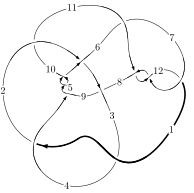
\includegraphics[width=112pt]{../../../GIT/diagram.site/Diagrams/png/1815_12a_1014.png}\\
\ \ \ A knot diagram\footnotemark}&
\allowdisplaybreaks
\textbf{Linearized knot diagam} \\
\cline{2-2}
 &
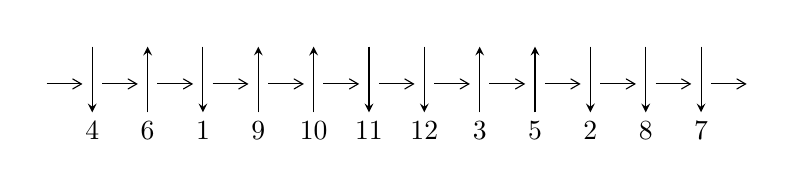
\begin{tikzpicture}[x=20pt, y=17pt]
	% nodes
	\node (C0) at (0, 0) {};
	\node (C1) at (1, 0) {};
	\node (C1U) at (1, +1) {};
	\node (C1D) at (1, -1) {4};

	\node (C2) at (2, 0) {};
	\node (C2U) at (2, +1) {};
	\node (C2D) at (2, -1) {6};

	\node (C3) at (3, 0) {};
	\node (C3U) at (3, +1) {};
	\node (C3D) at (3, -1) {1};

	\node (C4) at (4, 0) {};
	\node (C4U) at (4, +1) {};
	\node (C4D) at (4, -1) {9};

	\node (C5) at (5, 0) {};
	\node (C5U) at (5, +1) {};
	\node (C5D) at (5, -1) {10};

	\node (C6) at (6, 0) {};
	\node (C6U) at (6, +1) {};
	\node (C6D) at (6, -1) {11};

	\node (C7) at (7, 0) {};
	\node (C7U) at (7, +1) {};
	\node (C7D) at (7, -1) {12};

	\node (C8) at (8, 0) {};
	\node (C8U) at (8, +1) {};
	\node (C8D) at (8, -1) {3};

	\node (C9) at (9, 0) {};
	\node (C9U) at (9, +1) {};
	\node (C9D) at (9, -1) {5};

	\node (C10) at (10, 0) {};
	\node (C10U) at (10, +1) {};
	\node (C10D) at (10, -1) {2};

	\node (C11) at (11, 0) {};
	\node (C11U) at (11, +1) {};
	\node (C11D) at (11, -1) {8};

	\node (C12) at (12, 0) {};
	\node (C12U) at (12, +1) {};
	\node (C12D) at (12, -1) {7};
	\node (C13) at (13, 0) {};

	% arrows
	\draw[->,>={angle 60}]
	(C0) edge (C1) (C1) edge (C2) (C2) edge (C3) (C3) edge (C4) (C4) edge (C5) (C5) edge (C6) (C6) edge (C7) (C7) edge (C8) (C8) edge (C9) (C9) edge (C10) (C10) edge (C11) (C11) edge (C12) (C12) edge (C13) ;	\draw[->,>=stealth]
	(C1U) edge (C1D) (C2D) edge (C2U) (C3U) edge (C3D) (C4D) edge (C4U) (C5D) edge (C5U) (C6U) edge (C6D) (C7U) edge (C7D) (C8D) edge (C8U) (C9D) edge (C9U) (C10U) edge (C10D) (C11U) edge (C11D) (C12U) edge (C12D) ;
	\end{tikzpicture} \\
\hhline{~~} \\& 
\textbf{Solving Sequence} \\ \cline{2-2} 
 &
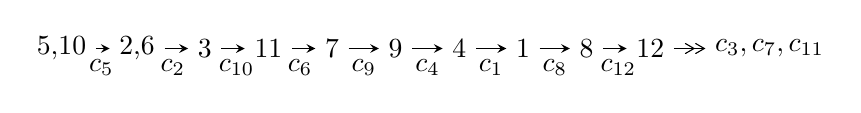
\begin{tikzpicture}[x=23pt, y=7pt]
	% node
	\node (A0) at (-1/8, 0) {5,10};
	\node (A1) at (17/16, 0) {2,6};
	\node (A2) at (17/8, 0) {3};
	\node (A3) at (25/8, 0) {11};
	\node (A4) at (33/8, 0) {7};
	\node (A5) at (41/8, 0) {9};
	\node (A6) at (49/8, 0) {4};
	\node (A7) at (57/8, 0) {1};
	\node (A8) at (65/8, 0) {8};
	\node (A9) at (73/8, 0) {12};
	\node (C1) at (1/2, -1) {$c_{5}$};
	\node (C2) at (13/8, -1) {$c_{2}$};
	\node (C3) at (21/8, -1) {$c_{10}$};
	\node (C4) at (29/8, -1) {$c_{6}$};
	\node (C5) at (37/8, -1) {$c_{9}$};
	\node (C6) at (45/8, -1) {$c_{4}$};
	\node (C7) at (53/8, -1) {$c_{1}$};
	\node (C8) at (61/8, -1) {$c_{8}$};
	\node (C9) at (69/8, -1) {$c_{12}$};
	\node (A10) at (11, 0) {$c_{3},c_{7},c_{11}$};

	% edge
	\draw[->,>=stealth]	
	(A0) edge (A1) (A1) edge (A2) (A2) edge (A3) (A3) edge (A4) (A4) edge (A5) (A5) edge (A6) (A6) edge (A7) (A7) edge (A8) (A8) edge (A9) ;
	\draw[->>,>={angle 60}]	
	(A9) edge (A10);
\end{tikzpicture} \\ 

\end{tabular} \\

\footnotetext{
The image of knot diagram is generated by the software ``\textbf{Draw programme}" developed by Andrew Bartholomew(\url{http://www.layer8.co.uk/maths/draw/index.htm\#Running-draw}), where we modified some parts for our purpose(\url{https://github.com/CATsTAILs/LinksPainter}).
}\phantom \\ \newline 
\centering \textbf{Ideals for irreducible components\footnotemark of $X_{\text{par}}$} 
 
\begin{align*}
I^u_{1}&=\langle 
-2.48028\times10^{137} u^{87}-1.90470\times10^{137} u^{86}+\cdots+7.25646\times10^{137} b+2.50630\times10^{137},\\
\phantom{I^u_{1}}&\phantom{= \langle  }2.11941\times10^{137} u^{87}+7.24817\times10^{137} u^{86}+\cdots+7.25646\times10^{137} a-8.34303\times10^{136},\;u^{88}+2 u^{87}+\cdots+4 u^2+1\rangle \\
I^u_{2}&=\langle 
7 b- u+2,\;7 a-3 u-1,\;u^2+u+1\rangle \\
\\
\end{align*}
\raggedright * 2 irreducible components of $\dim_{\mathbb{C}}=0$, with total 90 representations.\\
\footnotetext{All coefficients of polynomials are rational numbers. But the coefficients are sometimes approximated in decimal forms when there is not enough margin.}
\newpage
\renewcommand{\arraystretch}{1}
\centering \section*{I. $I^u_{1}= \langle -2.48\times10^{137} u^{87}-1.90\times10^{137} u^{86}+\cdots+7.26\times10^{137} b+2.51\times10^{137},\;2.12\times10^{137} u^{87}+7.25\times10^{137} u^{86}+\cdots+7.26\times10^{137} a-8.34\times10^{136},\;u^{88}+2 u^{87}+\cdots+4 u^2+1 \rangle$}
\flushleft \textbf{(i) Arc colorings}\\
\begin{tabular}{m{7pt} m{180pt} m{7pt} m{180pt} }
\flushright $a_{5}=$&$\begin{pmatrix}1\\0\end{pmatrix}$ \\
\flushright $a_{10}=$&$\begin{pmatrix}0\\u\end{pmatrix}$ \\
\flushright $a_{2}=$&$\begin{pmatrix}-0.292072 u^{87}-0.998857 u^{86}+\cdots+4.58008 u+0.114974\\0.341803 u^{87}+0.262483 u^{86}+\cdots-0.159539 u-0.345389\end{pmatrix}$ \\
\flushright $a_{6}=$&$\begin{pmatrix}1\\- u^2\end{pmatrix}$ \\
\flushright $a_{3}=$&$\begin{pmatrix}-0.264668 u^{87}-0.894639 u^{86}+\cdots+4.71261 u+0.184298\\0.325117 u^{87}+0.233773 u^{86}+\cdots-0.132136 u-0.295978\end{pmatrix}$ \\
\flushright $a_{11}=$&$\begin{pmatrix}-0.138518 u^{87}+2.23892 u^{86}+\cdots-0.340831 u-3.88428\\3.10091 u^{87}+1.52591 u^{86}+\cdots-1.72649 u+2.45169\end{pmatrix}$ \\
\flushright $a_{7}=$&$\begin{pmatrix}-0.963044 u^{87}-0.180143 u^{86}+\cdots+3.28975 u+3.23650\\2.30375 u^{87}+1.20769 u^{86}+\cdots-1.34975 u+1.52417\end{pmatrix}$ \\
\flushright $a_{9}=$&$\begin{pmatrix}- u\\u\end{pmatrix}$ \\
\flushright $a_{4}=$&$\begin{pmatrix}- u^2+1\\u^2\end{pmatrix}$ \\
\flushright $a_{1}=$&$\begin{pmatrix}-0.215669 u^{87}-0.801951 u^{86}+\cdots+4.52640 u-1.04103\\0.321531 u^{87}+0.203061 u^{86}+\cdots-0.215669 u-0.370612\end{pmatrix}$ \\
\flushright $a_{8}=$&$\begin{pmatrix}2.84777 u^{87}+3.42425 u^{86}+\cdots-8.89289 u-1.49021\\-3.51383 u^{87}-2.67370 u^{86}+\cdots+1.69517 u-2.18337\end{pmatrix}$ \\
\flushright $a_{12}=$&$\begin{pmatrix}0.209783 u^{87}+1.31979 u^{86}+\cdots+1.71885 u-2.35314\\1.79542 u^{87}+1.30105 u^{86}+\cdots-0.315595 u+1.00197\end{pmatrix}$\\&\end{tabular}
\flushleft \textbf{(ii) Obstruction class $= -1$}\\~\\
\flushleft \textbf{(iii) Cusp Shapes $= -3.67403 u^{87}-4.82309 u^{86}+\cdots-7.57749 u-3.42504$}\\~\\
\newpage\renewcommand{\arraystretch}{1}
\flushleft \textbf{(iv) u-Polynomials at the component}\newline \\
\begin{tabular}{m{50pt}|m{274pt}}
Crossings & \hspace{64pt}u-Polynomials at each crossing \\
\hline $$\begin{aligned}c_{1},c_{3}\end{aligned}$$&$\begin{aligned}
&u^{88}-3 u^{87}+\cdots-295 u+49
\end{aligned}$\\
\hline $$\begin{aligned}c_{2}\end{aligned}$$&$\begin{aligned}
&u^{88}-7 u^{87}+\cdots-980 u+196
\end{aligned}$\\
\hline $$\begin{aligned}c_{4},c_{5},c_{9}\end{aligned}$$&$\begin{aligned}
&u^{88}+2 u^{87}+\cdots+4 u^2+1
\end{aligned}$\\
\hline $$\begin{aligned}c_{6}\end{aligned}$$&$\begin{aligned}
&u^{88}-2 u^{87}+\cdots-218 u+65
\end{aligned}$\\
\hline $$\begin{aligned}c_{7},c_{11},c_{12}\end{aligned}$$&$\begin{aligned}
&u^{88}+2 u^{87}+\cdots+2 u+1
\end{aligned}$\\
\hline $$\begin{aligned}c_{8}\end{aligned}$$&$\begin{aligned}
&7(7 u^{88}-36 u^{87}+\cdots-40832 u+4553)
\end{aligned}$\\
\hline $$\begin{aligned}c_{10}\end{aligned}$$&$\begin{aligned}
&7(7 u^{88}+71 u^{87}+\cdots+449 u+1459)
\end{aligned}$\\
\hline
\end{tabular}\\~\\
\newpage\renewcommand{\arraystretch}{1}
\flushleft \textbf{(v) Riley Polynomials at the component}\newline \\
\begin{tabular}{m{50pt}|m{274pt}}
Crossings & \hspace{64pt}Riley Polynomials at each crossing \\
\hline $$\begin{aligned}c_{1},c_{3}\end{aligned}$$&$\begin{aligned}
&y^{88}-53 y^{87}+\cdots-18915 y+2401
\end{aligned}$\\
\hline $$\begin{aligned}c_{2}\end{aligned}$$&$\begin{aligned}
&y^{88}-15 y^{87}+\cdots-201880 y+38416
\end{aligned}$\\
\hline $$\begin{aligned}c_{4},c_{5},c_{9}\end{aligned}$$&$\begin{aligned}
&y^{88}-82 y^{87}+\cdots+8 y+1
\end{aligned}$\\
\hline $$\begin{aligned}c_{6}\end{aligned}$$&$\begin{aligned}
&y^{88}-34 y^{87}+\cdots+196616 y+4225
\end{aligned}$\\
\hline $$\begin{aligned}c_{7},c_{11},c_{12}\end{aligned}$$&$\begin{aligned}
&y^{88}+74 y^{87}+\cdots+8 y+1
\end{aligned}$\\
\hline $$\begin{aligned}c_{8}\end{aligned}$$&$\begin{aligned}
&49(49 y^{88}+3926 y^{87}+\cdots-8.10942\times10^{8} y+2.07298\times10^{7})
\end{aligned}$\\
\hline $$\begin{aligned}c_{10}\end{aligned}$$&$\begin{aligned}
&49(49 y^{88}+4003 y^{87}+\cdots-2854063 y+2128681)
\end{aligned}$\\
\hline
\end{tabular}\\~\\
\newpage\flushleft \textbf{(vi) Complex Volumes and Cusp Shapes}
$$\begin{array}{c|c|c}  
\text{Solutions to }I^u_{1}& \I (\text{vol} + \sqrt{-1}CS) & \text{Cusp shape}\\
 \hline 
\begin{aligned}
u &= \phantom{-}0.465025 + 0.870255 I \\
a &= \phantom{-}0.208785 + 1.159280 I \\
b &= \phantom{-}0.309065 - 0.370721 I\end{aligned}
 & -2.82358 + 4.12952 I & \phantom{-0.000000 } 0 \\ \hline\begin{aligned}
u &= \phantom{-}0.465025 - 0.870255 I \\
a &= \phantom{-}0.208785 - 1.159280 I \\
b &= \phantom{-}0.309065 + 0.370721 I\end{aligned}
 & -2.82358 - 4.12952 I & \phantom{-0.000000 } 0 \\ \hline\begin{aligned}
u &= \phantom{-}0.678542 + 0.774022 I \\
a &= -0.907312 + 0.128470 I \\
b &= \phantom{-}0.806388 + 0.235769 I\end{aligned}
 & \phantom{-}0.40735 - 7.71051 I & \phantom{-0.000000 } 0 \\ \hline\begin{aligned}
u &= \phantom{-}0.678542 - 0.774022 I \\
a &= -0.907312 - 0.128470 I \\
b &= \phantom{-}0.806388 - 0.235769 I\end{aligned}
 & \phantom{-}0.40735 + 7.71051 I & \phantom{-0.000000 } 0 \\ \hline\begin{aligned}
u &= -0.474169 + 0.840049 I \\
a &= \phantom{-}0.241987 - 1.390130 I \\
b &= \phantom{-}0.299699 + 0.471165 I\end{aligned}
 & -5.23953 - 8.76456 I & \phantom{-0.000000 } 0 \\ \hline\begin{aligned}
u &= -0.474169 - 0.840049 I \\
a &= \phantom{-}0.241987 + 1.390130 I \\
b &= \phantom{-}0.299699 - 0.471165 I\end{aligned}
 & -5.23953 + 8.76456 I & \phantom{-0.000000 } 0 \\ \hline\begin{aligned}
u &= \phantom{-}0.475214 + 0.823836 I \\
a &= \phantom{-}0.31410 + 1.52013 I \\
b &= \phantom{-}0.268780 - 0.528112 I\end{aligned}
 & -0.16472 + 13.04760 I & \phantom{-0.000000 } 0 \\ \hline\begin{aligned}
u &= \phantom{-}0.475214 - 0.823836 I \\
a &= \phantom{-}0.31410 - 1.52013 I \\
b &= \phantom{-}0.268780 + 0.528112 I\end{aligned}
 & -0.16472 - 13.04760 I & \phantom{-0.000000 } 0 \\ \hline\begin{aligned}
u &= \phantom{-}0.224097 + 1.032390 I \\
a &= \phantom{-}0.478233 + 0.326886 I \\
b &= \phantom{-}0.155332 - 0.081088 I\end{aligned}
 & -1.55925 + 2.49981 I & \phantom{-0.000000 } 0 \\ \hline\begin{aligned}
u &= \phantom{-}0.224097 - 1.032390 I \\
a &= \phantom{-}0.478233 - 0.326886 I \\
b &= \phantom{-}0.155332 + 0.081088 I\end{aligned}
 & -1.55925 - 2.49981 I & \phantom{-0.000000 } 0\\
 \hline 
 \end{array}$$\newpage$$\begin{array}{c|c|c}  
\text{Solutions to }I^u_{1}& \I (\text{vol} + \sqrt{-1}CS) & \text{Cusp shape}\\
 \hline 
\begin{aligned}
u &= -0.709608 + 0.809911 I \\
a &= -0.732695 - 0.187189 I \\
b &= \phantom{-}0.708824 - 0.197729 I\end{aligned}
 & -4.61019 + 3.28116 I & \phantom{-0.000000 } 0 \\ \hline\begin{aligned}
u &= -0.709608 - 0.809911 I \\
a &= -0.732695 + 0.187189 I \\
b &= \phantom{-}0.708824 + 0.197729 I\end{aligned}
 & -4.61019 - 3.28116 I & \phantom{-0.000000 } 0 \\ \hline\begin{aligned}
u &= -0.355788 + 0.802924 I \\
a &= \phantom{-}0.877968 - 0.955168 I \\
b &= \phantom{-}0.043536 + 0.303056 I\end{aligned}
 & \phantom{-}5.68213 - 4.42760 I & \phantom{-0.000000 } 0 \\ \hline\begin{aligned}
u &= -0.355788 - 0.802924 I \\
a &= \phantom{-}0.877968 + 0.955168 I \\
b &= \phantom{-}0.043536 - 0.303056 I\end{aligned}
 & \phantom{-}5.68213 + 4.42760 I & \phantom{-0.000000 } 0 \\ \hline\begin{aligned}
u &= \phantom{-}0.807583 + 0.884999 I \\
a &= -0.454813 + 0.140604 I \\
b &= \phantom{-}0.533679 + 0.217858 I\end{aligned}
 & -2.00805 + 1.65292 I & \phantom{-0.000000 } 0 \\ \hline\begin{aligned}
u &= \phantom{-}0.807583 - 0.884999 I \\
a &= -0.454813 - 0.140604 I \\
b &= \phantom{-}0.533679 - 0.217858 I\end{aligned}
 & -2.00805 - 1.65292 I & \phantom{-0.000000 } 0 \\ \hline\begin{aligned}
u &= -0.590432 + 0.529783 I \\
a &= -0.598808 + 0.811973 I \\
b &= \phantom{-}0.588467 - 0.662727 I\end{aligned}
 & \phantom{-}6.79240 + 0.03358 I & \phantom{-}6.01227 + 1.06957 I \\ \hline\begin{aligned}
u &= -0.590432 - 0.529783 I \\
a &= -0.598808 - 0.811973 I \\
b &= \phantom{-}0.588467 + 0.662727 I\end{aligned}
 & \phantom{-}6.79240 - 0.03358 I & \phantom{-}6.01227 - 1.06957 I \\ \hline\begin{aligned}
u &= -1.248020 + 0.027660 I \\
a &= \phantom{-}0.971817 + 0.039767 I \\
b &= \phantom{-}0.385149 + 0.317525 I\end{aligned}
 & \phantom{-}1.89898 - 3.61624 I & \phantom{-0.000000 } 0 \\ \hline\begin{aligned}
u &= -1.248020 - 0.027660 I \\
a &= \phantom{-}0.971817 - 0.039767 I \\
b &= \phantom{-}0.385149 - 0.317525 I\end{aligned}
 & \phantom{-}1.89898 + 3.61624 I & \phantom{-0.000000 } 0\\
 \hline 
 \end{array}$$\newpage$$\begin{array}{c|c|c}  
\text{Solutions to }I^u_{1}& \I (\text{vol} + \sqrt{-1}CS) & \text{Cusp shape}\\
 \hline 
\begin{aligned}
u &= \phantom{-}1.25038\phantom{ +0.000000I} \\
a &= \phantom{-}1.00048\phantom{ +0.000000I} \\
b &= \phantom{-}0.302083\phantom{ +0.000000I}\end{aligned}
 & -2.00769\phantom{ +0.000000I} & \phantom{-0.000000 } 0 \\ \hline\begin{aligned}
u &= \phantom{-}0.428355 + 0.546083 I \\
a &= -0.42999 - 1.60423 I \\
b &= \phantom{-}0.289935 + 1.063610 I\end{aligned}
 & \phantom{-}3.81209 + 7.45383 I & \phantom{-}1.39315 - 8.57538 I \\ \hline\begin{aligned}
u &= \phantom{-}0.428355 - 0.546083 I \\
a &= -0.42999 + 1.60423 I \\
b &= \phantom{-}0.289935 - 1.063610 I\end{aligned}
 & \phantom{-}3.81209 - 7.45383 I & \phantom{-}1.39315 + 8.57538 I \\ \hline\begin{aligned}
u &= \phantom{-}1.313290 + 0.118441 I \\
a &= \phantom{-}0.193456 + 0.100801 I \\
b &= \phantom{-}0.78076 - 1.74527 I\end{aligned}
 & \phantom{-}2.98306 + 0.50959 I & \phantom{-0.000000 } 0 \\ \hline\begin{aligned}
u &= \phantom{-}1.313290 - 0.118441 I \\
a &= \phantom{-}0.193456 - 0.100801 I \\
b &= \phantom{-}0.78076 + 1.74527 I\end{aligned}
 & \phantom{-}2.98306 - 0.50959 I & \phantom{-0.000000 } 0 \\ \hline\begin{aligned}
u &= -1.331540 + 0.136013 I \\
a &= -0.065593 - 0.153457 I \\
b &= \phantom{-}0.93450 + 1.99969 I\end{aligned}
 & -0.39006 - 4.02805 I & \phantom{-0.000000 } 0 \\ \hline\begin{aligned}
u &= -1.331540 - 0.136013 I \\
a &= -0.065593 + 0.153457 I \\
b &= \phantom{-}0.93450 - 1.99969 I\end{aligned}
 & -0.39006 + 4.02805 I & \phantom{-0.000000 } 0 \\ \hline\begin{aligned}
u &= -0.411528 + 0.511958 I \\
a &= -0.21256 + 1.56445 I \\
b &= \phantom{-}0.162302 - 0.967337 I\end{aligned}
 & -1.04299 - 3.88125 I & -3.63273 + 8.23421 I \\ \hline\begin{aligned}
u &= -0.411528 - 0.511958 I \\
a &= -0.21256 - 1.56445 I \\
b &= \phantom{-}0.162302 + 0.967337 I\end{aligned}
 & -1.04299 + 3.88125 I & -3.63273 - 8.23421 I \\ \hline\begin{aligned}
u &= \phantom{-}1.340780 + 0.150050 I \\
a &= -0.236604 + 0.147537 I \\
b &= \phantom{-}1.04400 - 2.12368 I\end{aligned}
 & \phantom{-}3.97725 + 7.70239 I & \phantom{-0.000000 } 0\\
 \hline 
 \end{array}$$\newpage$$\begin{array}{c|c|c}  
\text{Solutions to }I^u_{1}& \I (\text{vol} + \sqrt{-1}CS) & \text{Cusp shape}\\
 \hline 
\begin{aligned}
u &= \phantom{-}1.340780 - 0.150050 I \\
a &= -0.236604 - 0.147537 I \\
b &= \phantom{-}1.04400 + 2.12368 I\end{aligned}
 & \phantom{-}3.97725 - 7.70239 I & \phantom{-0.000000 } 0 \\ \hline\begin{aligned}
u &= \phantom{-}1.365900 + 0.082318 I \\
a &= \phantom{-}0.164386 + 0.923797 I \\
b &= \phantom{-}0.34928 - 2.67036 I\end{aligned}
 & \phantom{-}2.94649 + 2.04332 I & \phantom{-0.000000 } 0 \\ \hline\begin{aligned}
u &= \phantom{-}1.365900 - 0.082318 I \\
a &= \phantom{-}0.164386 - 0.923797 I \\
b &= \phantom{-}0.34928 + 2.67036 I\end{aligned}
 & \phantom{-}2.94649 - 2.04332 I & \phantom{-0.000000 } 0 \\ \hline\begin{aligned}
u &= -1.369380 + 0.013705 I \\
a &= \phantom{-}2.54977 - 0.95313 I \\
b &= -4.25386 + 2.03407 I\end{aligned}
 & \phantom{-}2.02967 - 0.01294 I & \phantom{-0.000000 } 0 \\ \hline\begin{aligned}
u &= -1.369380 - 0.013705 I \\
a &= \phantom{-}2.54977 + 0.95313 I \\
b &= -4.25386 - 2.03407 I\end{aligned}
 & \phantom{-}2.02967 + 0.01294 I & \phantom{-0.000000 } 0 \\ \hline\begin{aligned}
u &= \phantom{-}0.470844 + 0.373071 I \\
a &= \phantom{-}0.094395 - 0.945702 I \\
b &= \phantom{-}0.220554 + 0.530322 I\end{aligned}
 & \phantom{-}0.905268 + 0.924263 I & \phantom{-}4.02456 - 3.18187 I \\ \hline\begin{aligned}
u &= \phantom{-}0.470844 - 0.373071 I \\
a &= \phantom{-}0.094395 + 0.945702 I \\
b &= \phantom{-}0.220554 - 0.530322 I\end{aligned}
 & \phantom{-}0.905268 - 0.924263 I & \phantom{-}4.02456 + 3.18187 I \\ \hline\begin{aligned}
u &= \phantom{-}0.302426 + 0.510200 I \\
a &= \phantom{-}1.92897 + 0.17179 I \\
b &= -0.256677 - 0.037097 I\end{aligned}
 & \phantom{-}3.59262 - 4.05238 I & \phantom{-}1.82011 + 0.64734 I \\ \hline\begin{aligned}
u &= \phantom{-}0.302426 - 0.510200 I \\
a &= \phantom{-}1.92897 - 0.17179 I \\
b &= -0.256677 + 0.037097 I\end{aligned}
 & \phantom{-}3.59262 + 4.05238 I & \phantom{-}1.82011 - 0.64734 I \\ \hline\begin{aligned}
u &= -1.368850 + 0.325549 I \\
a &= -0.276046 + 0.686310 I \\
b &= \phantom{-}0.70201 - 1.59031 I\end{aligned}
 & \phantom{-}8.47086 + 0.96250 I & \phantom{-0.000000 } 0\\
 \hline 
 \end{array}$$\newpage$$\begin{array}{c|c|c}  
\text{Solutions to }I^u_{1}& \I (\text{vol} + \sqrt{-1}CS) & \text{Cusp shape}\\
 \hline 
\begin{aligned}
u &= -1.368850 - 0.325549 I \\
a &= -0.276046 - 0.686310 I \\
b &= \phantom{-}0.70201 + 1.59031 I\end{aligned}
 & \phantom{-}8.47086 - 0.96250 I & \phantom{-0.000000 } 0 \\ \hline\begin{aligned}
u &= \phantom{-}1.409890 + 0.029155 I \\
a &= -0.65909 + 5.45104 I \\
b &= \phantom{-}1.81784 - 11.09350 I\end{aligned}
 & \phantom{-}6.42235 - 2.77134 I & \phantom{-0.000000 } 0 \\ \hline\begin{aligned}
u &= \phantom{-}1.409890 - 0.029155 I \\
a &= -0.65909 - 5.45104 I \\
b &= \phantom{-}1.81784 + 11.09350 I\end{aligned}
 & \phantom{-}6.42235 + 2.77134 I & \phantom{-0.000000 } 0 \\ \hline\begin{aligned}
u &= -1.42533 + 0.08102 I \\
a &= -0.911301 - 0.787379 I \\
b &= \phantom{-}1.90182 + 2.04497 I\end{aligned}
 & \phantom{-}7.54516 - 3.10813 I & \phantom{-0.000000 } 0 \\ \hline\begin{aligned}
u &= -1.42533 - 0.08102 I \\
a &= -0.911301 + 0.787379 I \\
b &= \phantom{-}1.90182 - 2.04497 I\end{aligned}
 & \phantom{-}7.54516 + 3.10813 I & \phantom{-0.000000 } 0 \\ \hline\begin{aligned}
u &= \phantom{-}0.320807 + 0.471107 I \\
a &= \phantom{-}0.23879 - 1.74609 I \\
b &= -0.233979 + 0.856786 I\end{aligned}
 & \phantom{-}1.63354 + 0.85045 I & -1.53895 - 5.23910 I \\ \hline\begin{aligned}
u &= \phantom{-}0.320807 - 0.471107 I \\
a &= \phantom{-}0.23879 + 1.74609 I \\
b &= -0.233979 - 0.856786 I\end{aligned}
 & \phantom{-}1.63354 - 0.85045 I & -1.53895 + 5.23910 I \\ \hline\begin{aligned}
u &= -1.44185 + 0.14310 I \\
a &= -0.570195 - 0.619847 I \\
b &= \phantom{-}0.69295 + 2.11347 I\end{aligned}
 & \phantom{-}7.32098 - 3.04286 I & \phantom{-0.000000 } 0 \\ \hline\begin{aligned}
u &= -1.44185 - 0.14310 I \\
a &= -0.570195 + 0.619847 I \\
b &= \phantom{-}0.69295 - 2.11347 I\end{aligned}
 & \phantom{-}7.32098 + 3.04286 I & \phantom{-0.000000 } 0 \\ \hline\begin{aligned}
u &= -0.154069 + 0.519282 I \\
a &= \phantom{-}0.60767 + 1.59884 I \\
b &= -1.070580 - 0.771606 I\end{aligned}
 & -0.68368 - 5.30063 I & -6.18473 + 7.46843 I\\
 \hline 
 \end{array}$$\newpage$$\begin{array}{c|c|c}  
\text{Solutions to }I^u_{1}& \I (\text{vol} + \sqrt{-1}CS) & \text{Cusp shape}\\
 \hline 
\begin{aligned}
u &= -0.154069 - 0.519282 I \\
a &= \phantom{-}0.60767 - 1.59884 I \\
b &= -1.070580 + 0.771606 I\end{aligned}
 & -0.68368 + 5.30063 I & -6.18473 - 7.46843 I \\ \hline\begin{aligned}
u &= \phantom{-}1.46093 + 0.18393 I \\
a &= -0.577303 + 0.740047 I \\
b &= \phantom{-}0.18603 - 2.36742 I\end{aligned}
 & \phantom{-}5.02748 + 6.44830 I & \phantom{-0.000000 } 0 \\ \hline\begin{aligned}
u &= \phantom{-}1.46093 - 0.18393 I \\
a &= -0.577303 - 0.740047 I \\
b &= \phantom{-}0.18603 + 2.36742 I\end{aligned}
 & \phantom{-}5.02748 - 6.44830 I & \phantom{-0.000000 } 0 \\ \hline\begin{aligned}
u &= -1.46509 + 0.19462 I \\
a &= -0.579534 - 0.802604 I \\
b &= \phantom{-}0.04047 + 2.47187 I\end{aligned}
 & \phantom{-}9.9418 - 10.1764 I & \phantom{-0.000000 } 0 \\ \hline\begin{aligned}
u &= -1.46509 - 0.19462 I \\
a &= -0.579534 + 0.802604 I \\
b &= \phantom{-}0.04047 - 2.47187 I\end{aligned}
 & \phantom{-}9.9418 + 10.1764 I & \phantom{-0.000000 } 0 \\ \hline\begin{aligned}
u &= \phantom{-}0.122670 + 0.505532 I \\
a &= \phantom{-}0.52604 - 1.34952 I \\
b &= -1.130960 + 0.595578 I\end{aligned}
 & -4.89818 + 1.73906 I & -12.21356 - 4.35527 I \\ \hline\begin{aligned}
u &= \phantom{-}0.122670 - 0.505532 I \\
a &= \phantom{-}0.52604 + 1.34952 I \\
b &= -1.130960 - 0.595578 I\end{aligned}
 & -4.89818 - 1.73906 I & -12.21356 + 4.35527 I \\ \hline\begin{aligned}
u &= -1.47349 + 0.15116 I \\
a &= -0.509337 - 0.629558 I \\
b &= \phantom{-}0.34252 + 1.90298 I\end{aligned}
 & \phantom{-}7.23343 - 2.97184 I & \phantom{-0.000000 } 0 \\ \hline\begin{aligned}
u &= -1.47349 - 0.15116 I \\
a &= -0.509337 + 0.629558 I \\
b &= \phantom{-}0.34252 - 1.90298 I\end{aligned}
 & \phantom{-}7.23343 + 2.97184 I & \phantom{-0.000000 } 0 \\ \hline\begin{aligned}
u &= -0.079421 + 0.507840 I \\
a &= \phantom{-}0.548744 + 0.934759 I \\
b &= -1.259470 - 0.407517 I\end{aligned}
 & -1.26799 + 1.70875 I & -7.72525 - 0.49338 I\\
 \hline 
 \end{array}$$\newpage$$\begin{array}{c|c|c}  
\text{Solutions to }I^u_{1}& \I (\text{vol} + \sqrt{-1}CS) & \text{Cusp shape}\\
 \hline 
\begin{aligned}
u &= -0.079421 - 0.507840 I \\
a &= \phantom{-}0.548744 - 0.934759 I \\
b &= -1.259470 + 0.407517 I\end{aligned}
 & -1.26799 - 1.70875 I & -7.72525 + 0.49338 I \\ \hline\begin{aligned}
u &= \phantom{-}1.43573 + 0.38529 I \\
a &= -0.007478 - 0.595504 I \\
b &= \phantom{-}0.08476 + 1.51582 I\end{aligned}
 & \phantom{-}2.71814 + 2.73664 I & \phantom{-0.000000 } 0 \\ \hline\begin{aligned}
u &= \phantom{-}1.43573 - 0.38529 I \\
a &= -0.007478 + 0.595504 I \\
b &= \phantom{-}0.08476 - 1.51582 I\end{aligned}
 & \phantom{-}2.71814 - 2.73664 I & \phantom{-0.000000 } 0 \\ \hline\begin{aligned}
u &= -0.269583 + 0.412174 I \\
a &= \phantom{-}1.78564 + 0.30892 I \\
b &= -0.214649 - 0.070213 I\end{aligned}
 & -1.25437 + 0.85817 I & -4.51635 - 0.02662 I \\ \hline\begin{aligned}
u &= -0.269583 - 0.412174 I \\
a &= \phantom{-}1.78564 - 0.30892 I \\
b &= -0.214649 + 0.070213 I\end{aligned}
 & -1.25437 - 0.85817 I & -4.51635 + 0.02662 I \\ \hline\begin{aligned}
u &= \phantom{-}1.48155 + 0.30360 I \\
a &= \phantom{-}0.245807 - 1.043490 I \\
b &= -0.22891 + 2.56472 I\end{aligned}
 & \phantom{-}11.6500 + 8.4676 I & \phantom{-0.000000 } 0 \\ \hline\begin{aligned}
u &= \phantom{-}1.48155 - 0.30360 I \\
a &= \phantom{-}0.245807 + 1.043490 I \\
b &= -0.22891 - 2.56472 I\end{aligned}
 & \phantom{-}11.6500 - 8.4676 I & \phantom{-0.000000 } 0 \\ \hline\begin{aligned}
u &= \phantom{-}1.50563 + 0.17910 I \\
a &= -0.348456 + 0.721440 I \\
b &= -0.27315 - 1.84088 I\end{aligned}
 & \phantom{-}13.58050 + 2.56939 I & \phantom{-0.000000 } 0 \\ \hline\begin{aligned}
u &= \phantom{-}1.50563 - 0.17910 I \\
a &= -0.348456 - 0.721440 I \\
b &= -0.27315 + 1.84088 I\end{aligned}
 & \phantom{-}13.58050 - 2.56939 I & \phantom{-0.000000 } 0 \\ \hline\begin{aligned}
u &= \phantom{-}1.52367\phantom{ +0.000000I} \\
a &= -0.523082\phantom{ +0.000000I} \\
b &= \phantom{-}0.691833\phantom{ +0.000000I}\end{aligned}
 & \phantom{-}4.13126\phantom{ +0.000000I} & \phantom{-0.000000 } 0\\
 \hline 
 \end{array}$$\newpage$$\begin{array}{c|c|c}  
\text{Solutions to }I^u_{1}& \I (\text{vol} + \sqrt{-1}CS) & \text{Cusp shape}\\
 \hline 
\begin{aligned}
u &= -1.48453 + 0.34451 I \\
a &= \phantom{-}0.225794 + 0.730825 I \\
b &= -0.33907 - 1.91530 I\end{aligned}
 & \phantom{-}4.19421 - 7.28551 I & \phantom{-0.000000 } 0 \\ \hline\begin{aligned}
u &= -1.48453 - 0.34451 I \\
a &= \phantom{-}0.225794 - 0.730825 I \\
b &= -0.33907 + 1.91530 I\end{aligned}
 & \phantom{-}4.19421 + 7.28551 I & \phantom{-0.000000 } 0 \\ \hline\begin{aligned}
u &= \phantom{-}0.346362 + 0.322667 I \\
a &= \phantom{-}2.52356 - 1.29399 I \\
b &= -0.324707 + 0.186840 I\end{aligned}
 & \phantom{-}1.98288 + 1.74756 I & -0.63361 - 6.31369 I \\ \hline\begin{aligned}
u &= \phantom{-}0.346362 - 0.322667 I \\
a &= \phantom{-}2.52356 + 1.29399 I \\
b &= -0.324707 - 0.186840 I\end{aligned}
 & \phantom{-}1.98288 - 1.74756 I & -0.63361 + 6.31369 I \\ \hline\begin{aligned}
u &= -1.51013 + 0.31460 I \\
a &= \phantom{-}0.512292 + 0.870667 I \\
b &= -0.85109 - 2.34807 I\end{aligned}
 & \phantom{-}3.54515 - 8.41526 I & \phantom{-0.000000 } 0 \\ \hline\begin{aligned}
u &= -1.51013 - 0.31460 I \\
a &= \phantom{-}0.512292 - 0.870667 I \\
b &= -0.85109 + 2.34807 I\end{aligned}
 & \phantom{-}3.54515 + 8.41526 I & \phantom{-0.000000 } 0 \\ \hline\begin{aligned}
u &= -1.51365 + 0.29904 I \\
a &= \phantom{-}0.637562 + 1.039300 I \\
b &= -1.01287 - 2.74790 I\end{aligned}
 & \phantom{-}6.2721 - 17.1376 I & \phantom{-0.000000 } 0 \\ \hline\begin{aligned}
u &= -1.51365 - 0.29904 I \\
a &= \phantom{-}0.637562 - 1.039300 I \\
b &= -1.01287 + 2.74790 I\end{aligned}
 & \phantom{-}6.2721 + 17.1376 I & \phantom{-0.000000 } 0 \\ \hline\begin{aligned}
u &= \phantom{-}1.51356 + 0.30479 I \\
a &= \phantom{-}0.604525 - 0.961803 I \\
b &= -0.98748 + 2.57780 I\end{aligned}
 & \phantom{-}1.18596 + 12.92690 I & \phantom{-0.000000 } 0 \\ \hline\begin{aligned}
u &= \phantom{-}1.51356 - 0.30479 I \\
a &= \phantom{-}0.604525 + 0.961803 I \\
b &= -0.98748 - 2.57780 I\end{aligned}
 & \phantom{-}1.18596 - 12.92690 I & \phantom{-0.000000 } 0\\
 \hline 
 \end{array}$$\newpage$$\begin{array}{c|c|c}  
\text{Solutions to }I^u_{1}& \I (\text{vol} + \sqrt{-1}CS) & \text{Cusp shape}\\
 \hline 
\begin{aligned}
u &= -0.410125 + 0.089016 I \\
a &= \phantom{-}5.23763 + 1.01500 I \\
b &= -0.285000 - 0.082453 I\end{aligned}
 & \phantom{-}0.82913 + 3.21823 I & \phantom{-}9.71233 + 3.98519 I \\ \hline\begin{aligned}
u &= -0.410125 - 0.089016 I \\
a &= \phantom{-}5.23763 - 1.01500 I \\
b &= -0.285000 + 0.082453 I\end{aligned}
 & \phantom{-}0.82913 - 3.21823 I & \phantom{-}9.71233 - 3.98519 I \\ \hline\begin{aligned}
u &= \phantom{-}1.58966\phantom{ +0.000000I} \\
a &= -0.306266\phantom{ +0.000000I} \\
b &= \phantom{-}0.155878\phantom{ +0.000000I}\end{aligned}
 & \phantom{-}4.11849\phantom{ +0.000000I} & \phantom{-0.000000 } 0 \\ \hline\begin{aligned}
u &= \phantom{-}0.374898\phantom{ +0.000000I} \\
a &= \phantom{-}6.14886\phantom{ +0.000000I} \\
b &= -0.307864\phantom{ +0.000000I}\end{aligned}
 & -3.21214\phantom{ +0.000000I} & \phantom{-}11.9970\phantom{ +0.000000I} \\ \hline\begin{aligned}
u &= -1.61970 + 0.13613 I \\
a &= -0.090455 - 0.279218 I \\
b &= -0.411048 + 0.524774 I\end{aligned}
 & \phantom{-}8.41962 + 4.25598 I & \phantom{-0.000000 } 0 \\ \hline\begin{aligned}
u &= -1.61970 - 0.13613 I \\
a &= -0.090455 + 0.279218 I \\
b &= -0.411048 - 0.524774 I\end{aligned}
 & \phantom{-}8.41962 - 4.25598 I & \phantom{-0.000000 } 0 \\ \hline\begin{aligned}
u &= -0.132203 + 0.327967 I \\
a &= -0.85319 + 2.73462 I \\
b &= -0.650413 - 0.230842 I\end{aligned}
 & -1.78272 - 0.58271 I & -5.55303 - 2.81973 I \\ \hline\begin{aligned}
u &= -0.132203 - 0.327967 I \\
a &= -0.85319 - 2.73462 I \\
b &= -0.650413 + 0.230842 I\end{aligned}
 & -1.78272 + 0.58271 I & -5.55303 + 2.81973 I\\
 \hline 
 \end{array}$$\newpage\newpage\renewcommand{\arraystretch}{1}
\centering \section*{II. $I^u_{2}= \langle 7 b- u+2,\;7 a-3 u-1,\;u^2+u+1 \rangle$}
\flushleft \textbf{(i) Arc colorings}\\
\begin{tabular}{m{7pt} m{180pt} m{7pt} m{180pt} }
\flushright $a_{5}=$&$\begin{pmatrix}1\\0\end{pmatrix}$ \\
\flushright $a_{10}=$&$\begin{pmatrix}0\\u\end{pmatrix}$ \\
\flushright $a_{2}=$&$\begin{pmatrix}\frac{3}{7} u+\frac{1}{7}\\\frac{1}{7} u-\frac{2}{7}\end{pmatrix}$ \\
\flushright $a_{6}=$&$\begin{pmatrix}1\\u+1\end{pmatrix}$ \\
\flushright $a_{3}=$&$\begin{pmatrix}\frac{3}{7} u+\frac{1}{7}\\\frac{1}{7} u-\frac{2}{7}\end{pmatrix}$ \\
\flushright $a_{11}=$&$\begin{pmatrix}\frac{5}{49} u-\frac{3}{49}\\\frac{46}{49} u-\frac{8}{49}\end{pmatrix}$ \\
\flushright $a_{7}=$&$\begin{pmatrix}-\frac{8}{49} u+\frac{44}{49}\\-\frac{5}{49} u+\frac{3}{49}\end{pmatrix}$ \\
\flushright $a_{9}=$&$\begin{pmatrix}- u\\u\end{pmatrix}$ \\
\flushright $a_{4}=$&$\begin{pmatrix}u+2\\- u-1\end{pmatrix}$ \\
\flushright $a_{1}=$&$\begin{pmatrix}-\frac{4}{7} u-\frac{13}{7}\\\frac{8}{7} u+\frac{5}{7}\end{pmatrix}$ \\
\flushright $a_{8}=$&$\begin{pmatrix}-\frac{47}{49} u-\frac{11}{49}\\\frac{38}{49} u-\frac{13}{49}\end{pmatrix}$ \\
\flushright $a_{12}=$&$\begin{pmatrix}\frac{16}{49} u-\frac{39}{49}\\\frac{59}{49} u+\frac{43}{49}\end{pmatrix}$\\&\end{tabular}
\flushleft \textbf{(ii) Obstruction class $= 1$}\\~\\
\flushleft \textbf{(iii) Cusp Shapes $= \frac{52}{49} u+\frac{155}{49}$}\\~\\
\newpage\renewcommand{\arraystretch}{1}
\flushleft \textbf{(iv) u-Polynomials at the component}\newline \\
\begin{tabular}{m{50pt}|m{274pt}}
Crossings & \hspace{64pt}u-Polynomials at each crossing \\
\hline $$\begin{aligned}c_{1}\end{aligned}$$&$\begin{aligned}
&(u-1)^2
\end{aligned}$\\
\hline $$\begin{aligned}c_{2}\end{aligned}$$&$\begin{aligned}
&u^2
\end{aligned}$\\
\hline $$\begin{aligned}c_{3}\end{aligned}$$&$\begin{aligned}
&(u+1)^2
\end{aligned}$\\
\hline $$\begin{aligned}c_{4},c_{5},c_{6}\\c_{11},c_{12}\end{aligned}$$&$\begin{aligned}
&u^2+u+1
\end{aligned}$\\
\hline $$\begin{aligned}c_{7},c_{9}\end{aligned}$$&$\begin{aligned}
&u^2- u+1
\end{aligned}$\\
\hline $$\begin{aligned}c_{8}\end{aligned}$$&$\begin{aligned}
&7(7 u^2-3 u+3)
\end{aligned}$\\
\hline $$\begin{aligned}c_{10}\end{aligned}$$&$\begin{aligned}
&7(7 u^2-4 u+1)
\end{aligned}$\\
\hline
\end{tabular}\\~\\
\newpage\renewcommand{\arraystretch}{1}
\flushleft \textbf{(v) Riley Polynomials at the component}\newline \\
\begin{tabular}{m{50pt}|m{274pt}}
Crossings & \hspace{64pt}Riley Polynomials at each crossing \\
\hline $$\begin{aligned}c_{1},c_{3}\end{aligned}$$&$\begin{aligned}
&(y-1)^2
\end{aligned}$\\
\hline $$\begin{aligned}c_{2}\end{aligned}$$&$\begin{aligned}
&y^2
\end{aligned}$\\
\hline $$\begin{aligned}c_{4},c_{5},c_{6}\\c_{7},c_{9},c_{11}\\c_{12}\end{aligned}$$&$\begin{aligned}
&y^2+y+1
\end{aligned}$\\
\hline $$\begin{aligned}c_{8}\end{aligned}$$&$\begin{aligned}
&49(49 y^2+33 y+9)
\end{aligned}$\\
\hline $$\begin{aligned}c_{10}\end{aligned}$$&$\begin{aligned}
&49(49 y^2-2 y+1)
\end{aligned}$\\
\hline
\end{tabular}\\~\\
\newpage\flushleft \textbf{(vi) Complex Volumes and Cusp Shapes}
$$\begin{array}{c|c|c}  
\text{Solutions to }I^u_{2}& \I (\text{vol} + \sqrt{-1}CS) & \text{Cusp shape}\\
 \hline 
\begin{aligned}
u &= -0.500000 + 0.866025 I \\
a &= -0.071429 + 0.371154 I \\
b &= -0.357143 + 0.123718 I\end{aligned}
 & -1.64493 - 2.02988 I & \phantom{-}2.63265 + 0.91905 I \\ \hline\begin{aligned}
u &= -0.500000 - 0.866025 I \\
a &= -0.071429 - 0.371154 I \\
b &= -0.357143 - 0.123718 I\end{aligned}
 & -1.64493 + 2.02988 I & \phantom{-}2.63265 - 0.91905 I\\
 \hline 
 \end{array}$$\newpage
\newpage\renewcommand{\arraystretch}{1}
\centering \section*{ III. u-Polynomials}
\begin{tabular}{m{50pt}|m{274pt}}
Crossings & \hspace{64pt}u-Polynomials at each crossing \\
\hline $$\begin{aligned}c_{1}\end{aligned}$$&$\begin{aligned}
&((u-1)^2)(u^{88}-3 u^{87}+\cdots-295 u+49)
\end{aligned}$\\
\hline $$\begin{aligned}c_{2}\end{aligned}$$&$\begin{aligned}
&u^2(u^{88}-7 u^{87}+\cdots-980 u+196)
\end{aligned}$\\
\hline $$\begin{aligned}c_{3}\end{aligned}$$&$\begin{aligned}
&((u+1)^2)(u^{88}-3 u^{87}+\cdots-295 u+49)
\end{aligned}$\\
\hline $$\begin{aligned}c_{4},c_{5}\end{aligned}$$&$\begin{aligned}
&(u^2+u+1)(u^{88}+2 u^{87}+\cdots+4 u^2+1)
\end{aligned}$\\
\hline $$\begin{aligned}c_{6}\end{aligned}$$&$\begin{aligned}
&(u^2+u+1)(u^{88}-2 u^{87}+\cdots-218 u+65)
\end{aligned}$\\
\hline $$\begin{aligned}c_{7}\end{aligned}$$&$\begin{aligned}
&(u^2- u+1)(u^{88}+2 u^{87}+\cdots+2 u+1)
\end{aligned}$\\
\hline $$\begin{aligned}c_{8}\end{aligned}$$&$\begin{aligned}
&49(7 u^2-3 u+3)(7 u^{88}-36 u^{87}+\cdots-40832 u+4553)
\end{aligned}$\\
\hline $$\begin{aligned}c_{9}\end{aligned}$$&$\begin{aligned}
&(u^2- u+1)(u^{88}+2 u^{87}+\cdots+4 u^2+1)
\end{aligned}$\\
\hline $$\begin{aligned}c_{10}\end{aligned}$$&$\begin{aligned}
&49(7 u^2-4 u+1)(7 u^{88}+71 u^{87}+\cdots+449 u+1459)
\end{aligned}$\\
\hline $$\begin{aligned}c_{11},c_{12}\end{aligned}$$&$\begin{aligned}
&(u^2+u+1)(u^{88}+2 u^{87}+\cdots+2 u+1)
\end{aligned}$\\
\hline
\end{tabular}\newpage\renewcommand{\arraystretch}{1}
\centering \section*{ IV. Riley Polynomials}
\begin{tabular}{m{50pt}|m{274pt}}
Crossings & \hspace{64pt}Riley Polynomials at each crossing \\
\hline $$\begin{aligned}c_{1},c_{3}\end{aligned}$$&$\begin{aligned}
&((y-1)^2)(y^{88}-53 y^{87}+\cdots-18915 y+2401)
\end{aligned}$\\
\hline $$\begin{aligned}c_{2}\end{aligned}$$&$\begin{aligned}
&y^2(y^{88}-15 y^{87}+\cdots-201880 y+38416)
\end{aligned}$\\
\hline $$\begin{aligned}c_{4},c_{5},c_{9}\end{aligned}$$&$\begin{aligned}
&(y^2+y+1)(y^{88}-82 y^{87}+\cdots+8 y+1)
\end{aligned}$\\
\hline $$\begin{aligned}c_{6}\end{aligned}$$&$\begin{aligned}
&(y^2+y+1)(y^{88}-34 y^{87}+\cdots+196616 y+4225)
\end{aligned}$\\
\hline $$\begin{aligned}c_{7},c_{11},c_{12}\end{aligned}$$&$\begin{aligned}
&(y^2+y+1)(y^{88}+74 y^{87}+\cdots+8 y+1)
\end{aligned}$\\
\hline $$\begin{aligned}c_{8}\end{aligned}$$&$\begin{aligned}
&2401(49 y^2+33 y+9)\\
&\cdot(49 y^{88}+3926 y^{87}+\cdots-810942196 y+20729809)
\end{aligned}$\\
\hline $$\begin{aligned}c_{10}\end{aligned}$$&$\begin{aligned}
&2401(49 y^2-2 y+1)(49 y^{88}+4003 y^{87}+\cdots-2854063 y+2128681)
\end{aligned}$\\
\hline
\end{tabular}
\vskip 2pc
\end{document}